\question \textbf{Table representation}
  
An alignment can be represented as a table with arrows. Vertical and horizontal arrows indicate gaps, while diagonal arrows indicate matches and mismatches.

Identify the alignment that corresponds to the arrows in the following tables.
\medskip 

\begin{parts}

%% (a)
\part Table 1

\begin{figure}[h]
  \centering
      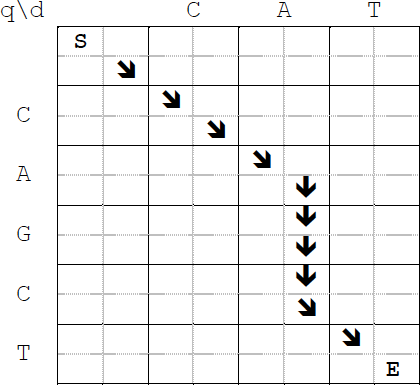
\includegraphics[width=0.325 \textwidth]{fig02/alignment_table_exercise_1.png}
\end{figure}

\begin{solution}[0.75 in]
\begin{verbatim}
  q: CAGCT
  d: CA--T
\end{verbatim}
\end{solution}

%% (b)
\part Table 2 

\begin{figure}[!h]
  \centering
      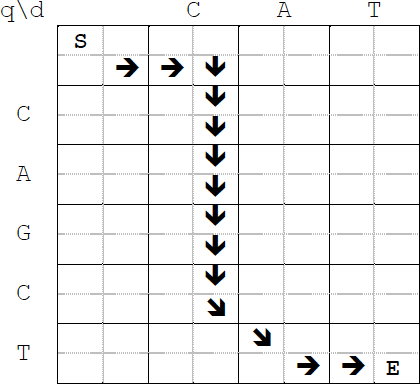
\includegraphics[width=0.325 \textwidth]{fig02/alignment_table_exercise_2.png}
\end{figure}

\begin{solution}[0.75 in]
\begin{verbatim}
  q: -CAGCT-
  d: C----AT
\end{verbatim}
\end{solution}

\end{parts}
